\part[Collections]{Collections}
\section{Overview of the Collections API}
\begin{frame}{Overview - Package Hierarchy}
\begin{center}
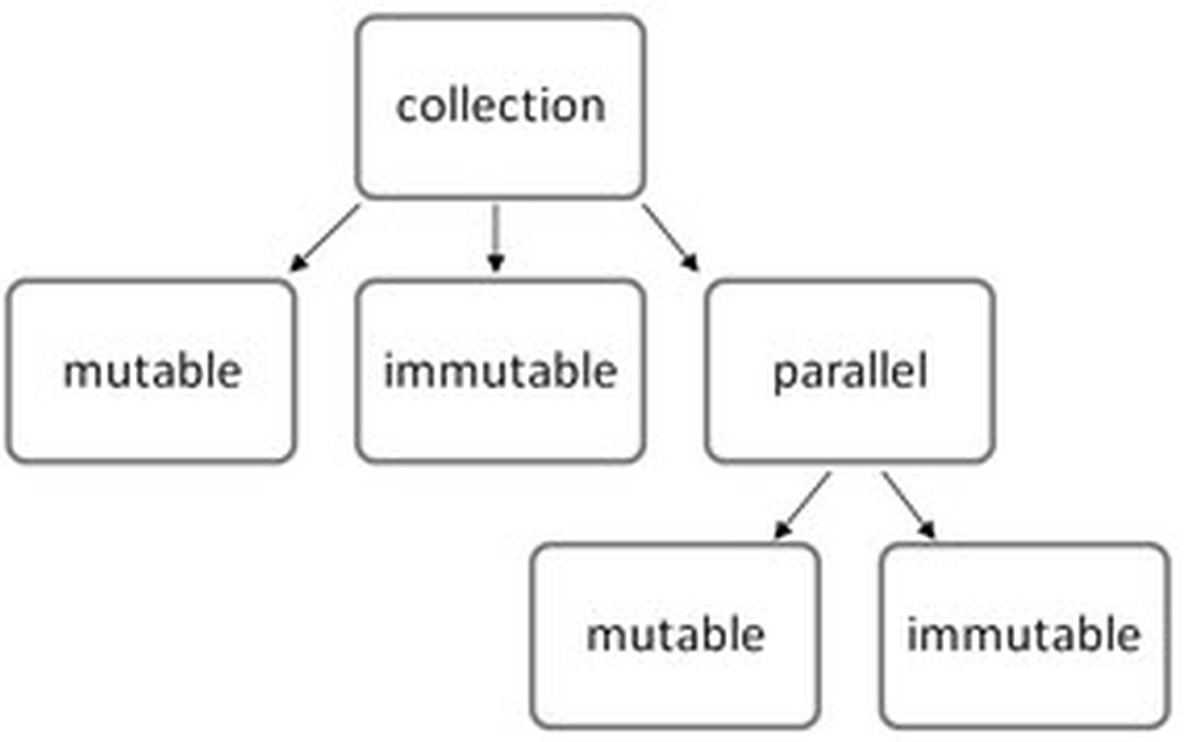
\includegraphics{resources/PackageHierarchy.jpg}
\end{center}
\end{frame}

\begin{frame}{Overview - Class Hierarchy}
\begin{center}
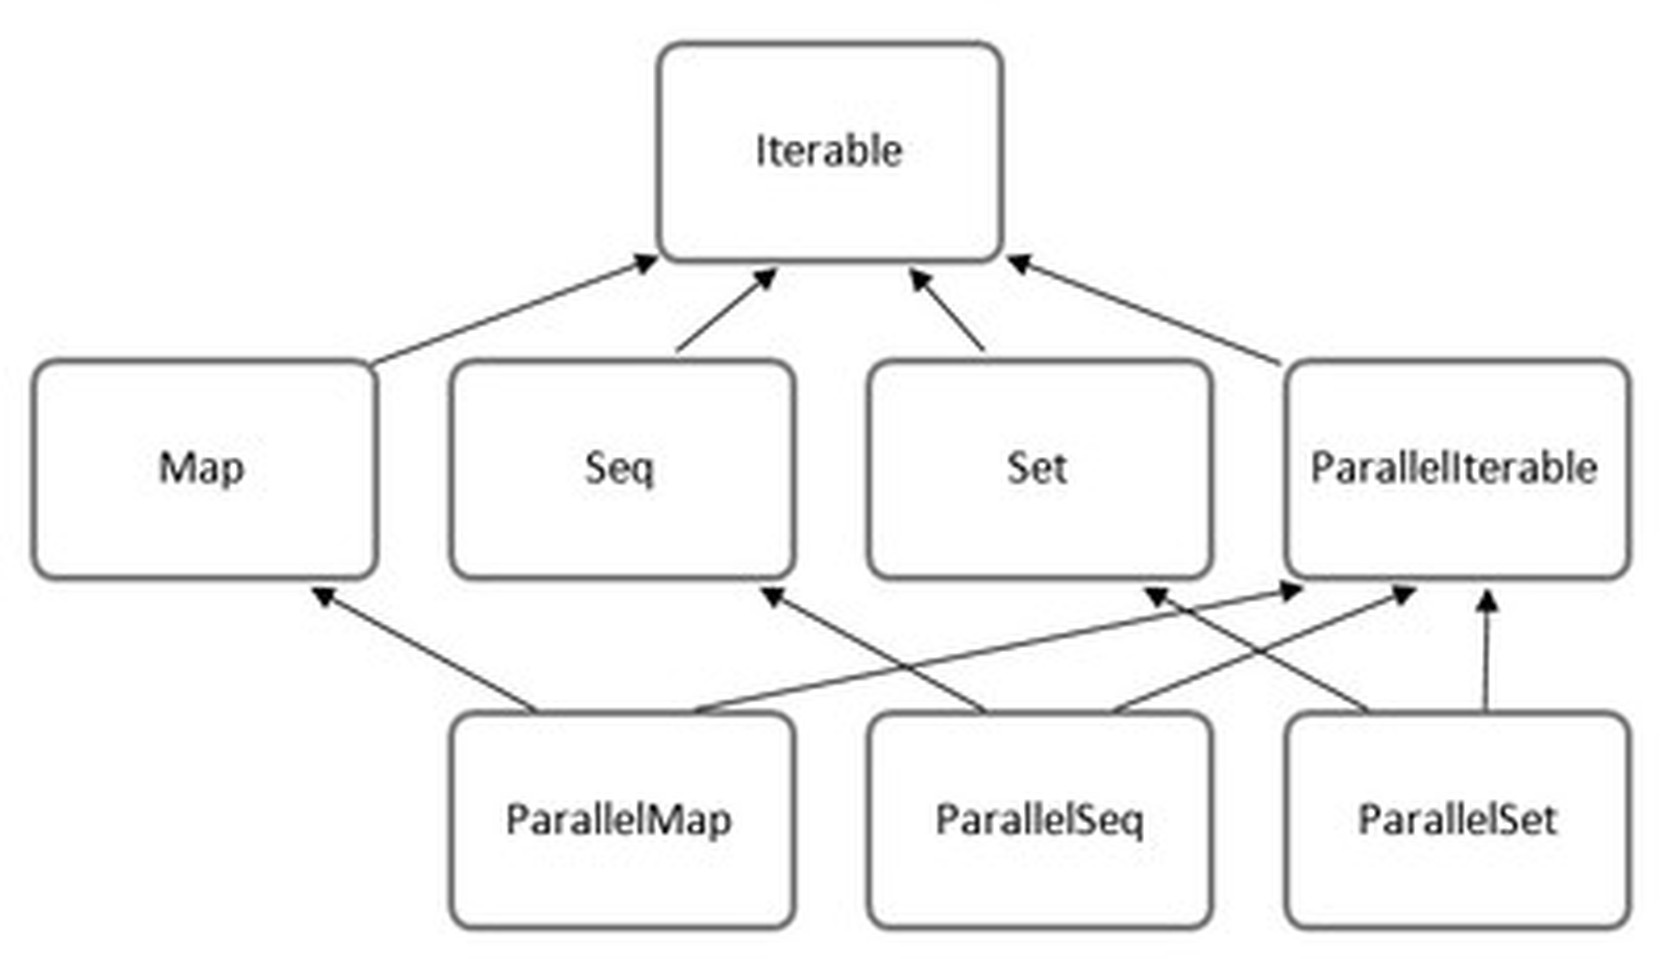
\includegraphics[width = 0.9\textwidth]{resources/ClassHierarchy.jpg}
\end{center}
\end{frame}

\begin{frame}{Overview - collection}
\begin{center}
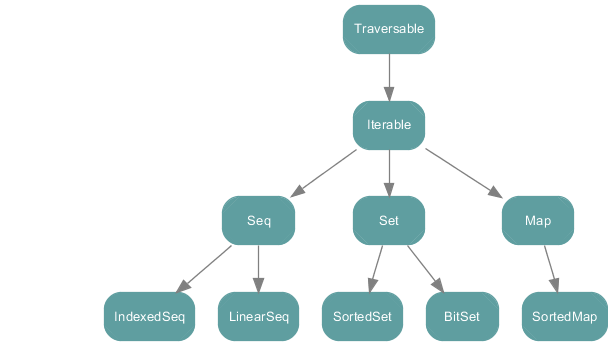
\includegraphics[width = \textwidth]{resources/collection.png}
\end{center}
\end{frame}

\begin{frame}{Overview - collection.immutable}
\begin{center}
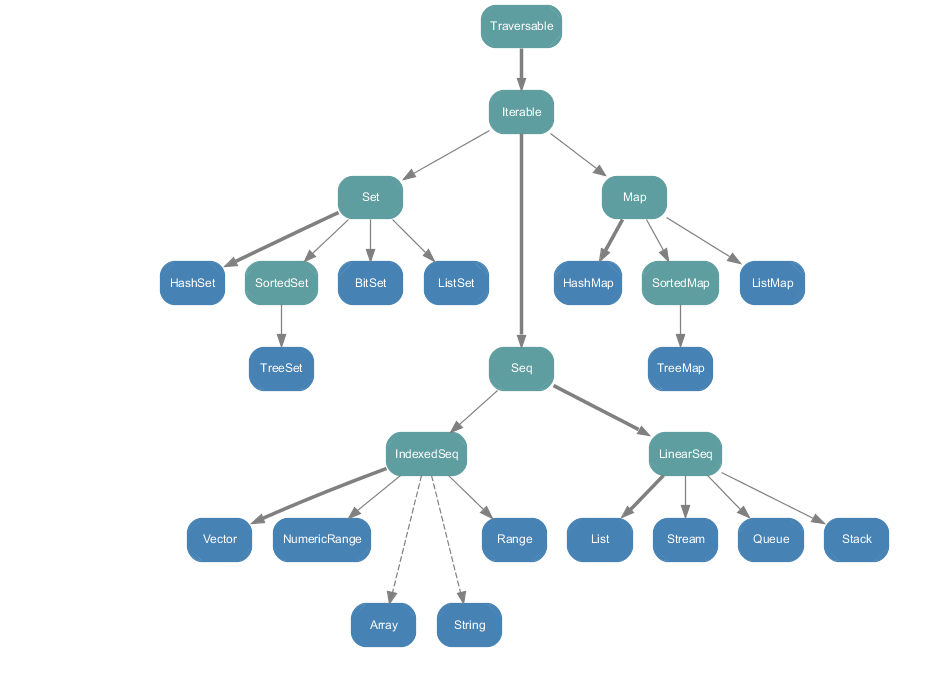
\includegraphics[width = \textwidth]{resources/collectionImmutable.png}
\end{center}
\end{frame}

\begin{frame}{Overview - collection.mutable}
\begin{center}
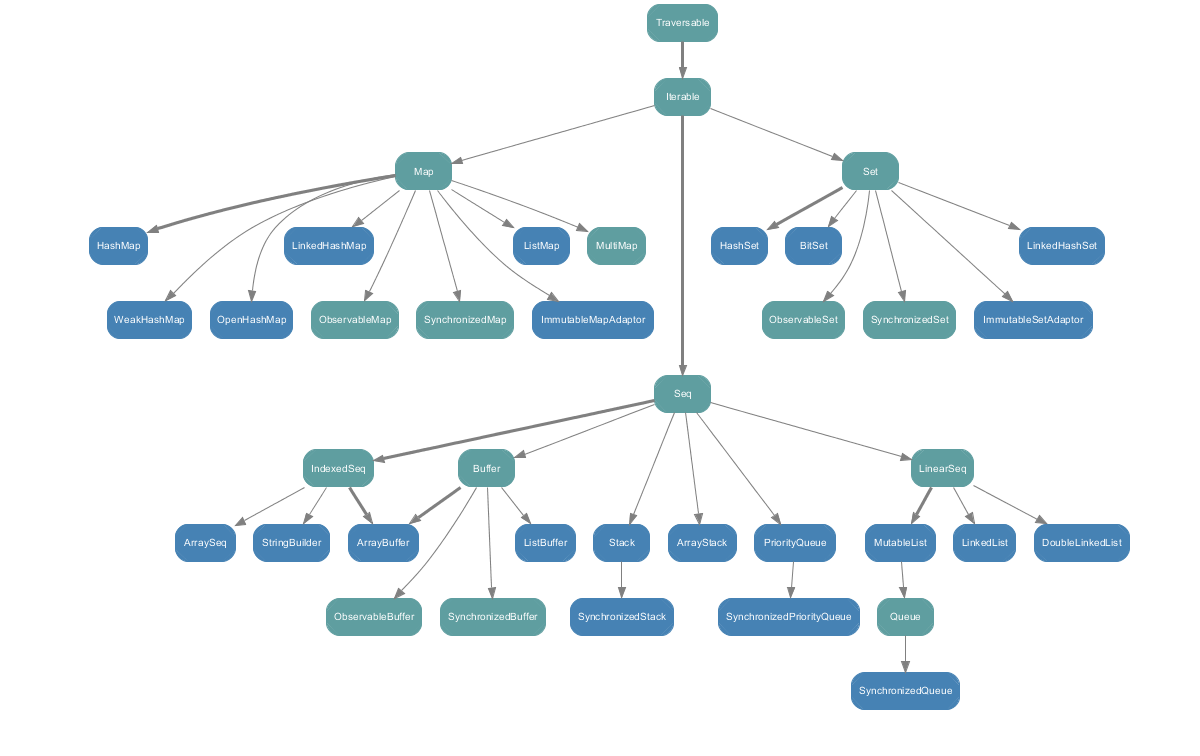
\includegraphics[width = \textwidth]{resources/collectionMutable.png}
\end{center}
\end{frame}

\begin{frame}{Overview - collection.parallel}
\begin{center}
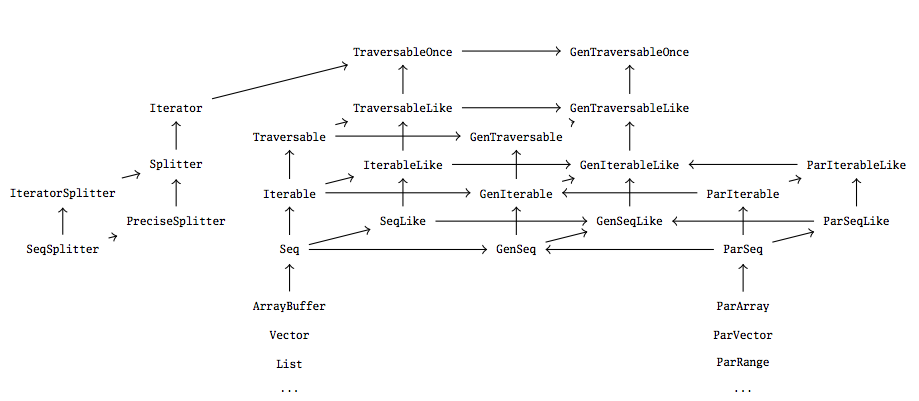
\includegraphics[width = \textwidth]{resources/collectionParallel.png}
\end{center}
\end{frame}

\begin{frame}[fragile]{Overview - Uniform syntax}
\begin{lstlisting}
Traversable(1, 2, 3)
Iterable("x", "y", "z")
Map("x" -> 24, "y" -> 25, "z" -> 26)
Set(Color.red, Color.green, Color.blue)
SortedSet("hello", "world")
Buffer(x, y, z)
IndexedSeq(1.0, 2.0)
LinearSeq(a, b, c) 
List(1, 2, 3)
HashMap("x" -> 24, "y" -> 25, "z" -> 26) 
\end{lstlisting}
\end{frame}

\begin{frame}[fragile]{Overview - Uniform return type principle}
\begin{lstlisting}
scala> List(1, 2, 3) map { _ + 1 }
res0: List[Int] = List(2, 3, 4)

scala> Set(1, 2, 3) map { _ + 1 }
res1: Set[Int] = Set(2, 3, 4) 
\end{lstlisting}
\end{frame}

\begin{frame}[fragile]{Overview - Type inference}
\begin{lstlisting}
import scala.collection.(im)mutable.HashMap

// no inference
val x: HashMap[String, Int] = new HashMap[String, Int]
val x: HashMap[String, Int] = HashMap[String, Int]()

// object inference
val x: HashMap[String, Int] = new HashMap
val x: HashMap[String, Int] = HashMap()

// reference inference
val x = new HashMap[String, Int]
val x = HashMap[String, Int]()

// full inference
val x = HashMap("dog" -> 3)
\end{lstlisting}
\end{frame}

\begin{frame}[fragile]{Overview - Trait Traversable}
\begin{center}
\lstinline!def foreach[U](f: Elem => U): Unit!
\end{center}
\begin{center}
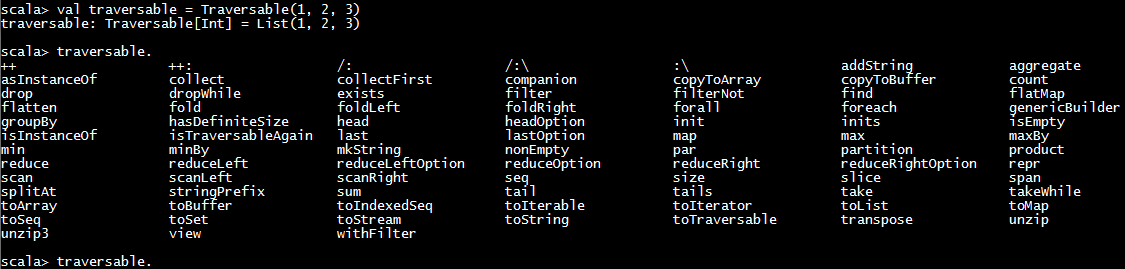
\includegraphics[width = \textwidth]{resources/Traversable.png}
\end{center}
\end{frame}

\begin{frame}[fragile]{Overview - Trait Iterable}
\begin{center}
\begin{lstlisting}
def foreach[U](f: Elem => U): Unit = {
  val it = iterator
  while (it.hasNext)
    f(it.next())
} 
\end{lstlisting}
\end{center}
\begin{center}
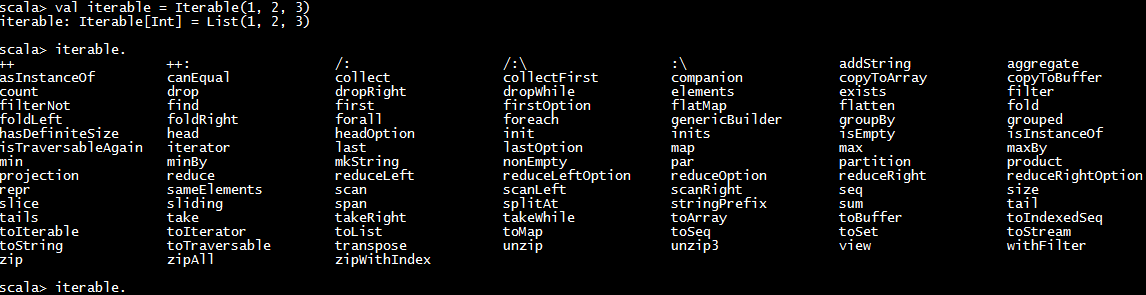
\includegraphics[width = \textwidth]{resources/Iterable.png}
\end{center}
\end{frame}

\begin{frame}[fragile]{Overview - Trait Iterable}
\begin{exampleblock}{grouped}
\begin{lstlisting}
scala> val xs = List(1, 2, 3, 4, 5)
xs: List[Int] = List(1, 2, 3, 4, 5)

scala> val git = xs grouped 3
git: Iterator[List[Int]] = non-empty iterator

scala> git.next()
res0: List[Int] = List(1, 2, 3)

scala> git.next()
res1: List[Int] = List(4, 5)
\end{lstlisting}
\end{exampleblock}
\end{frame}

\begin{frame}[fragile]{Overview - Trait Iterable}
\begin{exampleblock}{sliding}
\begin{lstlisting}
scala> val xs = List(1, 2, 3, 4, 5)
xs: List[Int] = List(1, 2, 3, 4, 5)

scala> val sit = xs sliding 3
sit: Iterator[List[Int]] = non-empty iterator

scala> sit.next()
res0: List[Int] = List(1, 2, 3)

scala> sit.next()
res1: List[Int] = List(2, 3, 4)

scala> sit.next()
res2: List[Int] = List(3, 4, 5) 
\end{lstlisting}
\end{exampleblock}
\end{frame}

\begin{frame}[fragile]{Overview - Seq, Set and Map}
\begin{exampleblock}{apply}
\begin{lstlisting}
scala> val seq = Seq(1, 2, 3)
seq: Seq[Int] = List(1, 2, 3)

scala> seq(1)
res0: Int = 2

scala> val set = Set(1, 2, 3)
set: Set[Int] = Set(1, 2, 3)

scala> set(1)
res1: Boolean = true

scala> val map = Map(1 -> "I", 2 -> "II", 3 -> "III")
map: Map[Int, java.lang.String] = Map(1 -> I, 2 -> II, 3 -> III)

scala> map(1)
res2: java.lang.String = I
\end{lstlisting}
\end{exampleblock}
\end{frame}

\begin{frame}[fragile]{Overview - Seq, IndexedSeq and LinearSeq}
The \lstinline!Seq trait! represents sequences. A \lstinline!Seq! is a kind of
\lstinline!Iterable! that has a \highlight{length} and whose elements have
\highlight{fixed index positions}, starting from 0.\\
\begin{center}
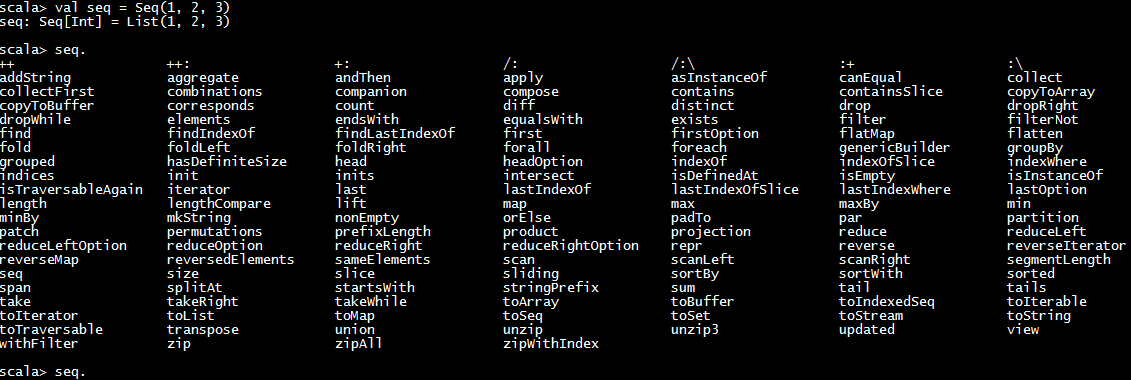
\includegraphics[width = \textwidth]{resources/Seq.png}
\end{center}
\end{frame}

\begin{frame}[fragile]{Overview - Seq, IndexedSeq and LinearSeq}
Trait \lstinline!Seq! has two subtraits: \lstinline!LinearSeq! and
\lstinline!IndexedSeq!. These do not add any new operations, but each offers
different performance characteristics: A linear sequence has efficient
\highlight{head and tail operations}, whereas an indexed sequence has efficient
\highlight{apply, length, and (if mutable) update operations}. Frequently used
linear sequences are \lstinline!immutable.List! and
\lstinline!immutable.Stream!. Frequently use  indexed sequences are
\lstinline!scala.Array! and \lstinline!mutable.ArrayBuffer!.
\newline
\newline
The \lstinline!Vector! class provides an interesting compromise between indexed
and linear access. It has \highlight{both effectively constant time indexing
overhead and constant time linear access overhead}. Because of this, vectors are
a good foundation for mixed access patterns where both indexed and linear
accesses are used.\\
\begin{center}
Use \lstinline!Vector! as your \highlight{default collection}
\end{center}
\end{frame}

\begin{frame}[fragile]{Overview - Sets}
\begin{center}
\lstinline!Set!s are \lstinline!Iterable!s that contain no duplicate elements
\end{center}
\begin{center}
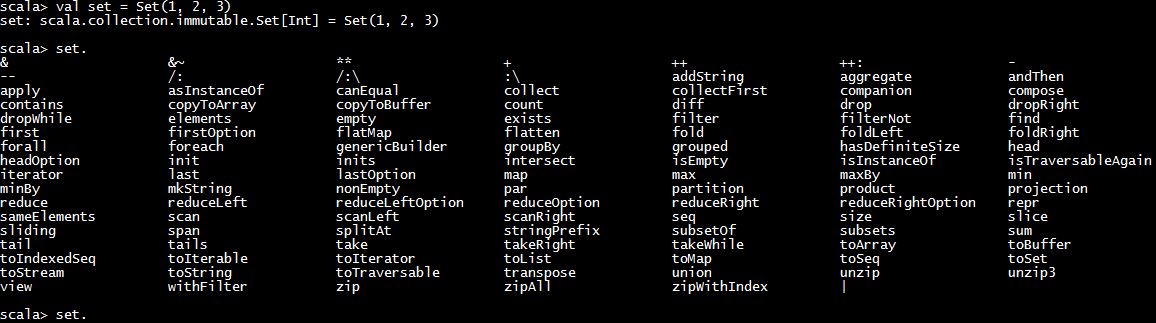
\includegraphics[width = \textwidth]{resources/Set.png}
\end{center}
\begin{lstlisting}
scala> val set = Set(1, 2, 3, 1, 2, 2, 4)
set: scala.collection.immutable.Set[Int] = Set(1, 2, 3, 4)
\end{lstlisting}
\end{frame}

\begin{frame}[fragile]{Overview - Maps}
A \lstinline!Map! is an \lstinline!Iterable! consisting of pairs of keys and
values (also named mappings or associations). Scala's \lstinline!Predef class!
offers an \highlight{implicit conversion} that lets you write \lstinline!key -> value! as
an alternate syntax for the pair \lstinline!(key, value)!.
\begin{center}
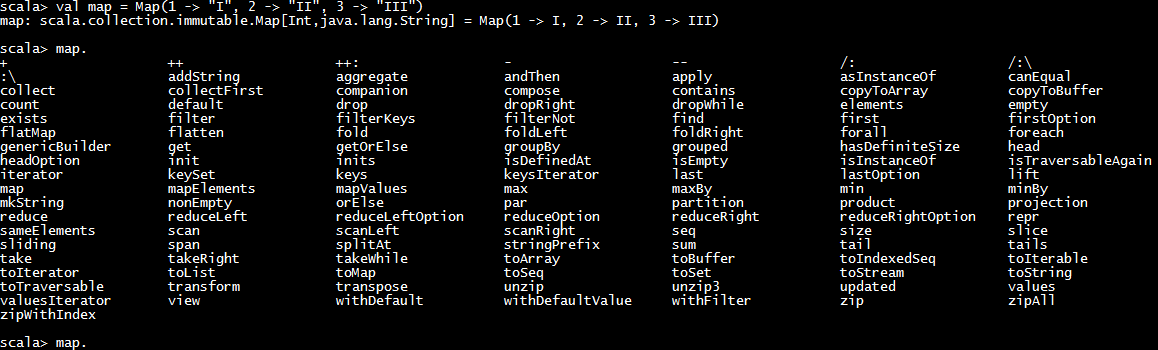
\includegraphics[width = \textwidth]{resources/Map.png}
\end{center}
\end{frame}

\section{Concrete Immutable Collection Classes}
\begin{frame}[fragile]{Streams}
A \lstinline!Stream! is like a \lstinline!List! except that its elements are
computed \lstinline!lazily!. Because of this, a stream can be
\lstinline!infinitely! long. Only those elements requested are computed.
Otherwise, streams have the same performance characteristics as lists.
\newline
\newline
Whereas lists are constructed with the \lstinline!::! operator, streams are
constructed with the similar-looking \lstinline!#::!. Here is a simple example
of a stream containing the integers 1, 2, and 3:\\
\begin{exampleblock}{\lstinline!Stream! - the lazy \lstinline!List!}
\begin{lstlisting}
scala> val str = 1 #:: 2 #:: 3 #:: Stream.empty
str: scala.collection.immutable.Stream[Int] = Stream(1, ?)
\end{lstlisting}
\end{exampleblock}
The head of this stream is 1, and the tail of it has 2 and 3. The tail is not
printed here, though, because it hasn't been computed yet! Streams are specified
to compute lazily, and the toString method of a stream is careful not to force
any extra evaluation.
\end{frame}

\begin{frame}[fragile]{Streams}
\begin{exampleblock}{Finite memory? Not a problem}
\begin{lstlisting}
scala> val ones: Stream[Int] = 1 #:: ones
ones: Stream[Int] = Stream(1, ?)

scala> ones take 10 foreach print
1111111111
\end{lstlisting}
\end{exampleblock}
\pause
\begin{exampleblock}{How many Fibonacci implementations are there? ;)}
\begin{lstlisting}
scala> def fib(a: Int, b: Int): Stream[Int] = a #:: fib(b, a + b)
fib: (a: Int, b: Int)Stream[Int]

scala> val fibs = fib(1, 1) take 7 toList
fibs: List[Int] = List(1, 1, 2, 3, 5, 8, 13)
\end{lstlisting}
\end{exampleblock}
\end{frame}

\begin{frame}[fragile]{Vectors}
\begin{lstlisting}
scala> val vec = Vector(1, 2, 3)
vec: immutable.Vector[Int] = Vector(1, 2, 3)

scala> val vec2 = vec :+ 4 :+ 5
vec2: immutable.Vector[Int] = Vector(1, 2, 3, 4, 5)

scala> val vec3 = 0 +: vec2
vec3: immutable.Vector[Int] = Vector(0, 1, 2, 3, 4, 5)

scala> val vec4 = vec3 updated (3, 6)
vec4: immutable.Vector[Int] = Vector(0, 1, 2, 6, 4, 5)

scala> vec3(3)
res6: Int = 3

scala> vec4(3)
res7: Int = 6
\end{lstlisting}
\end{frame}

\begin{frame}[fragile]{Ranges}
\begin{center}
A \lstinline!Range! is an ordered sequence of integers that are \highlight{equally spaced apart}
\end{center}
\begin{lstlisting}
scala> val range = 1 to 3
range: immutable.Range.Inclusive = Range(1, 2, 3)

scala> val range = 1 until 3
range: immutable.Range = Range(1, 2)

scala> val range = 1 to 10 by 3
range: immutable.Range = Range(1, 4, 7, 10)

scala> val range = 10 to 1 by -3
range: immutable.Range = Range(10, 7, 4, 1)
\end{lstlisting}
\end{frame}

\section{Performance Characteristics}
\begin{frame}{Performance characteristics}
\begin{center}
\begin{tabular}{|l|p{0.9\textwidth}|}
\hline
C & Constant time\\
\hline
eC & Effectively constant time, but this might depend on some assumptions such
as maximum length of a vector or distribution of hash keys.\\
\hline
aC & Amortized constant time. Some invocations might take longer, but if many
operations are performed on average only constant time per operation is taken.\\
\hline
Log & Time proportional to the logarithm of the collection size.\\
\hline
L & Linear time proportional to the collection size.\\
\hline
- & The operation is not supported.\\
\hline
\end{tabular}
\end{center}
\end{frame}
\begin{frame}{Performance characteristics of sequence types}
\begin{tabular}{|l|l|l|l|l|l|l|l|}
\hline
& head & tail & apply & update & prepend & append & insert\\
\hline
\highlight{immutable}\\
\hline
List & C & C & L & L & C & L & -\\
\hline
Stream & C & C & L & L & C & L & -\\
\hline
Vector & eC & eC & eC & eC & eC & eC & -\\
\hline
Stack & C & C & L & L & C & L & -\\
\hline
Queue & aC & aC & L & L & L & C & -\\
\hline
Range & C & C & C & - & - & - & -\\
\hline
String & C & L & C & L & L & L & -\\
\hline
\end{tabular}
\end{frame}

\begin{frame}{Performance characteristics of sequence types}
\begin{tabular}{|l|l|l|l|l|l|l|l|}
\hline
& head & tail & apply & update & prepend & append & insert\\
\hline
\highlight{mutable}\\
\hline
ArrayBuffer & C & L & C & C & L & aC & L\\
\hline
ListBuffer & C & L & L & L & C & C & L\\
\hline
StringBuilder & C & L & C & C & L & aC & L\\
\hline
MutableList & C & L & L & L & C & C & L\\
\hline
Queue & C & L & L & L & C & C & L\\
\hline
ArraySeq & C & L & C & C & - & - & -\\
\hline
Stack & C & L & L & L & C & L & L\\
\hline
ArrayStack & C & L & C & C & aC & L & L\\
\hline
Array & C & L & C & C & - & - & -\\
\hline
\end{tabular}
\end{frame}

\begin{frame}{Performance characteristics of set and map types}
\begin{tabular}{|l|l|l|l|l|}
\hline
& lookup & add & remove & min\\
\hline
\highlight{immutable}\\
\hline
HashSet/HashMap & eC & eC & eC & L\\
\hline
TreeSet/TreeMap & Log & Log & Log & Log\\
\hline
BitSet & C & L & L & eC\\
\hline
ListMap & L & L & L & L\\
\hline
\highlight{mutable}\\
\hline
HashSet/HashMap & eC & eC & eC & L\\
\hline
WeakHashMap & eC & eC & eC & L\\
\hline
BitSet & C & aC & C & eC\\
\hline
\end{tabular}
\end{frame}

\section{Views}
\section{Parallel Collections}
\section{Monadic for Comprehensions}

\section{Summary}
\begin{frame}{Summary}
\begin{itemize}
  \item
\end{itemize}
\end{frame}